% Data-preparation pipeline figure for the paper (data preparation section).
% Standalone TikZ -> compiles to data_pipeline.pdf (vector).
%   ../.tools/tectonic data_pipeline.tex   (from paper/figures/)
% Or \input / 
\includegraphics{figures/data_pipeline} inside main.tex.
\documentclass[border=6pt]{standalone}
\usepackage{tikz}
\usepackage{helvet}
\renewcommand{\familydefault}{\sfdefault}
\usetikzlibrary{positioning,arrows.meta,shapes.geometric,fit,backgrounds}

\begin{document}
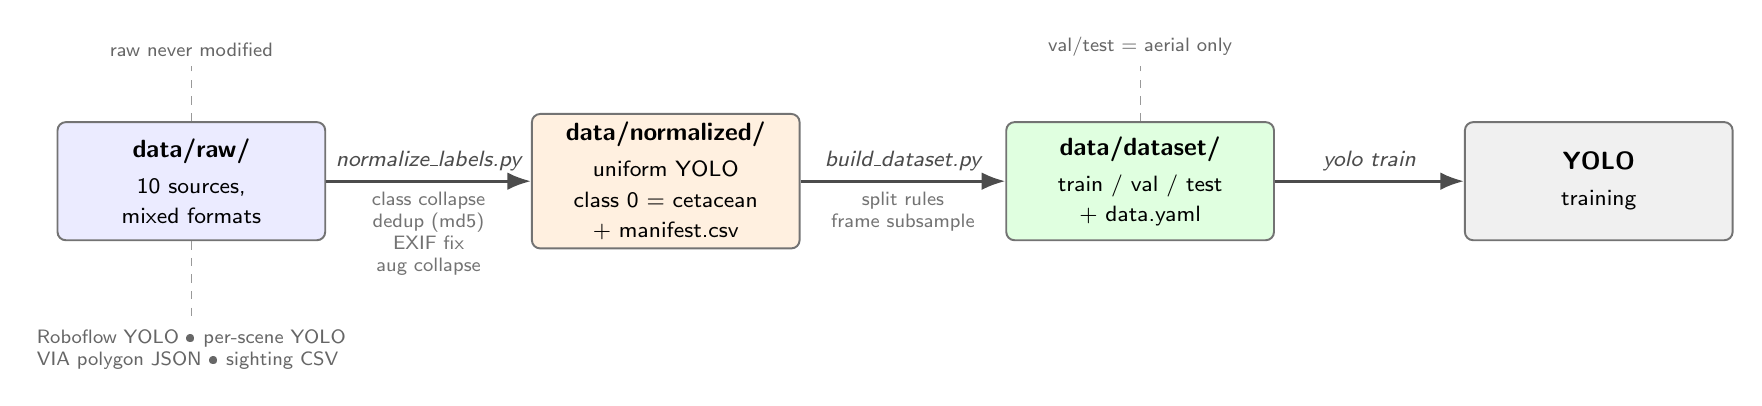
\begin{tikzpicture}[
  font=\small,
  stage/.style={rectangle, rounded corners=3pt, draw=black!55, line width=0.7pt,
                fill=#1, minimum width=34mm, minimum height=15mm, align=center,
                inner sep=3pt},
  script/.style={-{Stitch[]}, draw=black!70, line width=1pt},
  arrow/.style={-{Latex[length=3mm]}, line width=1pt, draw=black!70},
  lbl/.style={midway, above, font=\footnotesize\itshape, text=black!70},
  sub/.style={midway, below, font=\scriptsize, text=black!55, align=center},
  note/.style={font=\scriptsize, text=black!60, align=left},
]

% ---- main stage boxes ----
\node[stage=blue!8]  (raw)  {\textbf{data/raw/}\\[2pt]\footnotesize 10 sources,\\\footnotesize mixed formats};
\node[stage=orange!12] (norm) [right=26mm of raw]
      {\textbf{data/normalized/}\\[2pt]\footnotesize uniform YOLO\\\footnotesize class 0 = cetacean\\\footnotesize + manifest.csv};
\node[stage=green!12] (ds)  [right=26mm of norm]
      {\textbf{data/dataset/}\\[2pt]\footnotesize train / val / test\\\footnotesize + data.yaml};
\node[stage=black!6]  (train) [right=24mm of ds]
      {\textbf{YOLO}\\[2pt]\footnotesize training};

% ---- arrows with script labels ----
\draw[arrow] (raw)  -- node[lbl]{normalize\_labels.py}
                       node[sub]{class collapse\\dedup (md5)\\EXIF fix\\aug collapse} (norm);
\draw[arrow] (norm) -- node[lbl]{build\_dataset.py}
                       node[sub]{split rules\\frame subsample} (ds);
\draw[arrow] (ds)   -- node[lbl]{yolo train}  (train);

% ---- source-format callout under raw ----
\node[note] (fmts) [below=10mm of raw.south]
   {Roboflow YOLO \textbullet{} per-scene YOLO\\VIA polygon JSON \textbullet{} sighting CSV};
\draw[dashed, black!40] (raw.south) -- (fmts.north);

% ---- key-property callouts ----
\node[note] (rawprop) [above=7mm of raw.north] {raw never modified};
\draw[dashed, black!40] (raw.north) -- (rawprop.south);

\node[note] (dsprop) [above=7mm of ds.north] {val/test = aerial only};
\draw[dashed, black!40] (ds.north) -- (dsprop.south);

\end{tikzpicture}
\end{document}
